\chapter{Classic Architectures}
\label{ch:lesson37}

Chapters~\ref{ch:lesson34}--\ref{ch:lesson35} built and trained one small CNN. This chapter looks at how CNN \emph{architectures} evolved over roughly two decades, and works through the single biggest architectural idea in that history in detail: the \textbf{residual connection}, and the vanishing-gradient problem it was designed to fix.

\section{ImageNet and ILSVRC: the benchmark that drove this}

\textbf{ImageNet} (\citelink{deng2009}{Deng et al., 2009}) is a \emph{dataset}: over 14 million images, hand-labeled across more than 20,000 categories, built by crowdsourcing annotations onto WordNet's existing noun hierarchy. A big labeled dataset alone doesn't drive progress, though --- a shared, standardized \emph{competition} does. Starting in 2010, the \textbf{ILSVRC} (ImageNet Large Scale Visual Recognition Challenge, \citelink{russakovsky2015}{Russakovsky et al., 2015}) turned a 1000-category, $\sim$1.2-million-image subset of ImageNet into an annual benchmark: every group trained on the same data and was scored on the same held-out test set, making architectures directly, objectively comparable at a scale no one had managed before. The competition's winning top-5 error rate by year is a fair proxy for the field's progress across the decade this chapter covers:

\begin{center}
\renewcommand{\arraystretch}{1.3}
\begin{tabular}{lll}
\hline
\textbf{Year} & \textbf{Winner} & \textbf{Top-5 error} \\
\hline
2010 & (pre-deep-learning features)     & 28.2\% \\
2012 & AlexNet                          & 16.4\% \\
2014 & GoogLeNet (VGG close behind, at 7.3\%) & 6.7\% \\
2015 & ResNet                           & 3.57\% \\
2017 & SENet                            & 2.25\% \\
\hline
\end{tabular}
\end{center}

On this same task, a trained human achieves $\sim5\%$ error rate. ResNet was the first to beat this number --- sometimes referred to as ``super-human'' performance. By 2017, with the winning error under 2.5\%, ILSVRC's classification track was retired --- its job as a benchmark essentially done.

\section{A brief historical tour}

A handful of architectures were invented during this history, each solving a specific problem:
\begin{itemize}
  \item \textbf{LeNet-5} (\citelink{lecun1998}{LeCun et al., 1998}) --- the template Chapter~\ref{ch:lesson34} already implements: conv, pool, conv, pool, then fully-connected layers. Built for digit recognition on $32\times32$ images.
  \item \textbf{AlexNet} (\citelink{krizhevsky2012}{Krizhevsky, Sutskever \& Hinton, 2012}) --- the same template, just much bigger (5 conv layers, $\sim$60M parameters), trained on ImageNet using GPUs and ReLU instead of tanh/sigmoid. Its 2012 ILSVRC win is the watershed event that began the deep learning revolution in computer vision --- reviving mainstream interest in neural networks after a decade-long winter (akin to the ``AI winter'').
  \item \textbf{VGG} (\citelink{simonyanzisserman2014}{Simonyan \& Zisserman, 2015}) --- replaced AlexNet's large $11\times11$/$5\times5$ filters with a deep stack of small $3\times3$ convolutions. Two stacked $3\times3$ convs have the same \emph{receptive field} as one $5\times5$ conv (Chapter~\ref{ch:lesson11}'s pyramid idea again) but fewer parameters and an extra nonlinearity in between.
  \item \textbf{GoogLeNet / Inception} (\citelink{szegedy2015}{Szegedy et al., 2015}) --- went wider instead of just deeper: each ``Inception module'' runs several convolution sizes ($1\times1$, $3\times3$, $5\times5$) side by side on the same input and concatenates their outputs, so the network doesn't have to commit to one filter size per layer. $1\times1$ convolutions are used first to cheaply shrink the channel count, keeping the wider module affordable.
  \item \textbf{ResNet} (\citelink{he2015resnet}{He et al., 2016}) --- pushed depth from VGG's $\sim$19 layers to 50, 101, even 152, by solving the problem that had made naively stacking more layers \emph{worse}, not better.
  \item \textbf{SENet} (\citelink{hu2018senet}{Hu, Shen \& Sun, 2018}), the 2017 ILSVRC winner --- not a new backbone shape, but a refinement: its ``squeeze-and-excitation'' block lets each layer learn per-channel weights (which feature channels matter most for this input) rather than treating every channel equally.
\end{itemize}

The rest of this chapter focuses on ResNet's residual connection as the single most consequential idea in the table above.

\section{Building a ResNet block}

\subsection*{The vanishing-gradient problem}

Why does stacking more layers make plain networks \emph{worse}? Backprop's chain rule multiplies a gradient by every layer's local Jacobian on its way back to the input. If those per-layer factors are consistently smaller than 1 --- which happens easily with a saturating activation like sigmoid, whose derivative is at most 0.25 --- a deep enough stack multiplies the gradient by a very small number many times over. The gradient reaching early layers shrinks toward zero, and those layers stop learning at all.

Build a 30-layer, sigmoid-activated network of \code{Linear} layers and track the gradient magnitude at every depth, for two versions: a \textbf{plain} stack \code{x = sigmoid(layer(x))}, and a \textbf{residual} stack \code{x = x + 0.3 * sigmoid(layer(x))} where each layer only has to learn a small \emph{correction} added to its input, rather than replacing it outright.

\begin{lstlisting}
class ResidualDeepNet(nn.Module):
    def forward(self, x):
        for layer in self.layers:
            x = x + 0.3 * torch.sigmoid(layer(x))
        return x
\end{lstlisting}

For a 30-layer stack: the plain network's ratio of gradient norm at the input layer to the last layer is $2.07\times10^{-19}$; the residual network's ratio is $1.05\times10^0$ --- essentially flat (Figure~\ref{fig:l37-1}).

\begin{figure}[h]
\centering
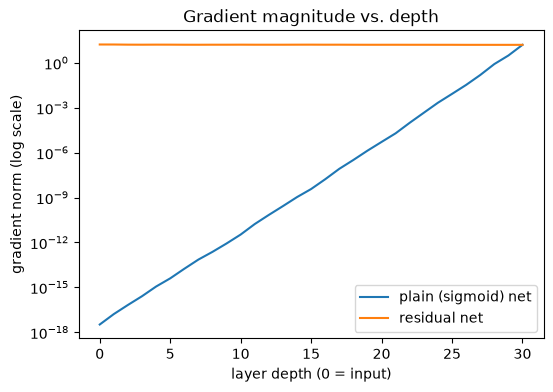
\includegraphics[width=0.6\textwidth]{figures/lesson37_fig01.png}
\caption{Gradient magnitude vs.\ depth, plain sigmoid network vs.\ residual network, log scale.}
\label{fig:l37-1}
\end{figure}

The plain network's gradient shrinks by roughly nineteen orders of magnitude between the last layer and the first --- for all practical purposes, the early layers receive no learning signal at all. The residual network's (ResNet's) gradient stays essentially flat across all 30 layers.

The reason is structural, not a matter of tuning: with a residual connection, $x_{l+1}=x_l+F(x_l)$, so $dx_{l+1}/dx_l=I+dF/dx_l$. Backprop multiplies these Jacobians together across layers, but every one of them contains an identity matrix $I$ as a direct term. That gives the gradient a path straight back to the input that never gets multiplied by a small sigmoid derivative --- an unobstructed shortcut, regardless of how deep the stack gets. The plain network has no such path: every layer's Jacobian is purely $dF/dx_l$, so there's nothing to stop repeated multiplication from driving the product toward zero.

\subsection*{Batch normalization}

ResNets use one more ingredient: \textbf{batch normalization} (\citelink{ioffeszegedy2015}{Ioffe \& Szegedy, 2015}). The idea is simple --- for each channel, subtract that channel's mean and divide by its standard deviation, computed \emph{across the current mini-batch} (over the batch, height, and width dimensions, separately per channel), so every channel's activations always have mean 0 and standard deviation 1 going into the next layer. Two learnable parameters, a per-channel scale $\gamma$ and shift $\beta$, are then applied on top, so the layer can still recover a different mean/scale if that's actually useful --- normalization to 0/1 is a \emph{starting point} the network can undo, not a hard constraint.

Deep networks without batch norm are prone to a related but distinct problem from vanishing gradients: as training updates early layers, the \emph{distribution} of activations feeding into later layers keeps shifting (sometimes called ``internal covariate shift''), so later layers are constantly chasing a moving target. Renormalizing at every layer keeps that distribution stable, which in practice lets much higher learning rates be used and makes deep networks noticeably easier to train --- one of the reasons ResNet could push to 50+ layers where earlier architectures struggled past $\sim$20.

A from-scratch per-channel normalize-then-scale-and-shift matches \code{nn.BatchNorm2d} to $4.77\times10^{-7}$: per-channel means and standard deviations that started at, e.g., $[-0.046, 0.165, -0.061, -0.165]$ and $[0.939, 1.037, 0.911, 0.977]$ come out at exactly $[0,0,0,0]$ and $[1,1,1,1]$ after normalization.

\subsection*{Putting it together: a convolutional residual block}

In an actual ResNet, $F$ is a pair of small convolutions (with batch normalization and ReLU in between), and the shortcut --- also called a \textbf{skip connection}, since it skips over $F$ entirely --- adds the \emph{input feature map} back onto their output, channel-for-channel and pixel-for-pixel:

\begin{lstlisting}
class ResidualBlock(nn.Module):
    def __init__(self, channels):
        super().__init__()
        self.conv1 = nn.Conv2d(channels, channels, 3, padding=1)
        self.bn1 = nn.BatchNorm2d(channels)
        self.conv2 = nn.Conv2d(channels, channels, 3, padding=1)
        self.bn2 = nn.BatchNorm2d(channels)

    def forward(self, x):
        out = torch.relu(self.bn1(self.conv1(x)))
        out = self.bn2(self.conv2(out))
        return torch.relu(x + out)  # the shortcut: add the block's input back in
\end{lstlisting}

Passing a $(4,16,20,20)$ tensor through the block produces an output of the identical shape $(4,16,20,20)$ --- a residual block preserves shape, so blocks can be stacked freely.

\subsection*{Exercises}
\begin{enumerate}
  \item In \code{PlainDeepNet}/\code{ResidualDeepNet} above, change the activation from \code{torch.sigmoid} to \code{torch.relu} (ReLU's derivative is 1 for any positive input, not capped at 0.25 like sigmoid's) and rerun the gradient-norm comparison. Does the plain network's vanishing problem get better, worse, or stay about the same?
  \item Change the residual net's scale factor from \code{0.3} to \code{1.0} (i.e.\ \code{x + torch.sigmoid(layer(x))} with no damping) and rerun. Does the gradient ratio change much? What does that suggest about \emph{why} the residual connection works --- is it the scale factor, or the \code{+ x} shortcut itself?
  \item \code{ResidualBlock} above requires the input and output to have the same number of channels, since they're added directly. Real ResNets sometimes need to change channel count between blocks (e.g.\ 16 $\to$ 32). Sketch (in words, or in code) what the shortcut path would need to do in that case for the addition to still make sense.
\end{enumerate}

\vfill
\fullcode{lesson37}{lesson37_classic_architectures}
